\chapter{Design and Implementation}
\begin{quote} 
\it This chapter covers the implementation details of the concept, the algorithms. All the simulations were first carried out in MATLAB{\textregistered} and Simulink{\textregistered}, testing and verifying.The section also introduces the proposed hybrid algorithm.
\end{quote}
%\right 

\section{Cell Characterisation}\label{sec:cel_char}
In this section, Model of two types of cells (\ac{a-Si} and \ac{DSCs}) is discussed.There are several Models that have been analysed in literature which are usually variations of the Single Diode model or the Double Diode model (discussed in section \ref{sec:SDM},\ref{sec:DDM} and \ref{sec:eDDM}).
 
\subsection{Test Setup}

 In the pursuance of creating a working solar cell model and to validate the algorithm several measurements would need to be performed. The Test-rig consisted of a blacked out enclosure to suppress interference from ambient light. The Test-rig or Light-box is fitted with an array of evenly spaced White-\ac{LED}s to provide uniform illumination on the Test subject. The \ac{LED}-array are calibrated and temperature controlled so as to provide white light with a known spectra. A high precision Lux Meter(\textit{GOSSEN Mavolux 5032B}) is used to measure the  intensity of the light, as perceived by the human eye. The \textit{GOSSEN} serves as a reference for Lux measurement throughout the project. The Light chamber is also routinely calibrated against a reference cell to factor-in the variations and degradation of the \ac{LED}s. The intensity of light is varied using a High-Voltage power source. A pictorial representation of the above description can be seen is figure ~\ref{fig:test setup} on page ~\pageref{fig:test setup}. \\



 \begin{figure}[H]
	  \begin{center}
		  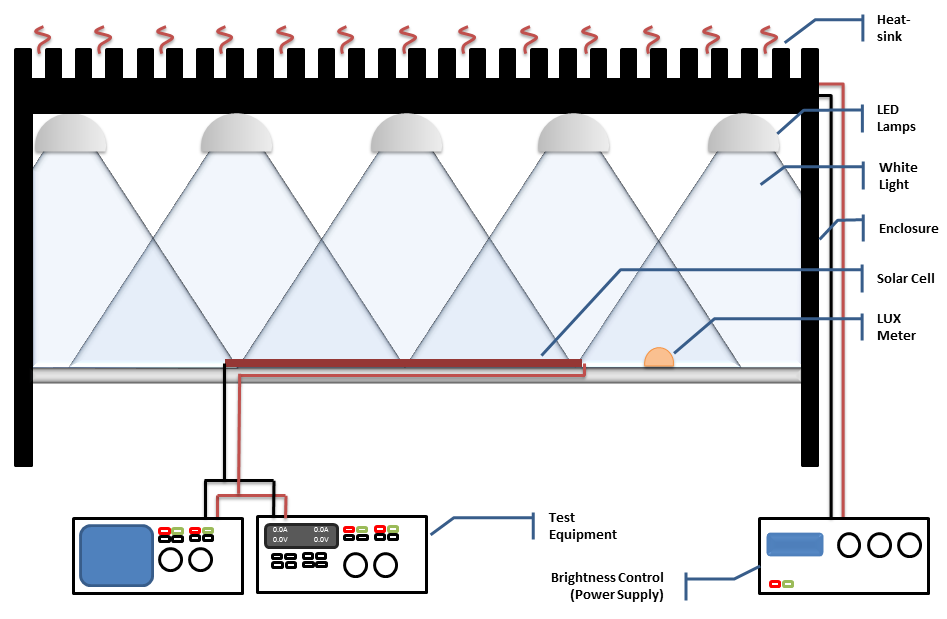
\includegraphics[width=\textwidth]{images/Light_Box}
		  \caption{Test Setup }
		  \label{fig:test setup}
	  \end{center}
  \end{figure}
  

Electrical models for solar cells are frequently found in literature \cite{vignati2012solutions} and \cite{yong2008modeling} among others -discussed in section \ref{sec:SDM} to \ref{sec:eDDM}.However \ac{DSCs} come in may different flavours:- dissimilar electrolytes \& electrodes; additional layers and junctions. Added to this fact, due to the near impossibility of accurately measuring the multitude of variables of a unknown cell, for this research work, a model was constructed by placing a the test cell under a battery of varied illuminations (0 Lux - 5050 Lux) shown in figure ~\ref{fig:Voltagevlux}. Which resulted in a surface that closely resembles the cell's operation under real world conditions. Particular attention was paid to low light conditions which is to be expected for indoor illuminations ( < 2000 Lux).As \ac{DSCs} display are very stable output across temperature ranges found indoor \cite{lee2010high}, the above model was made independent of temperature variations.

 \begin{figure}[H]
  \begin{center}
	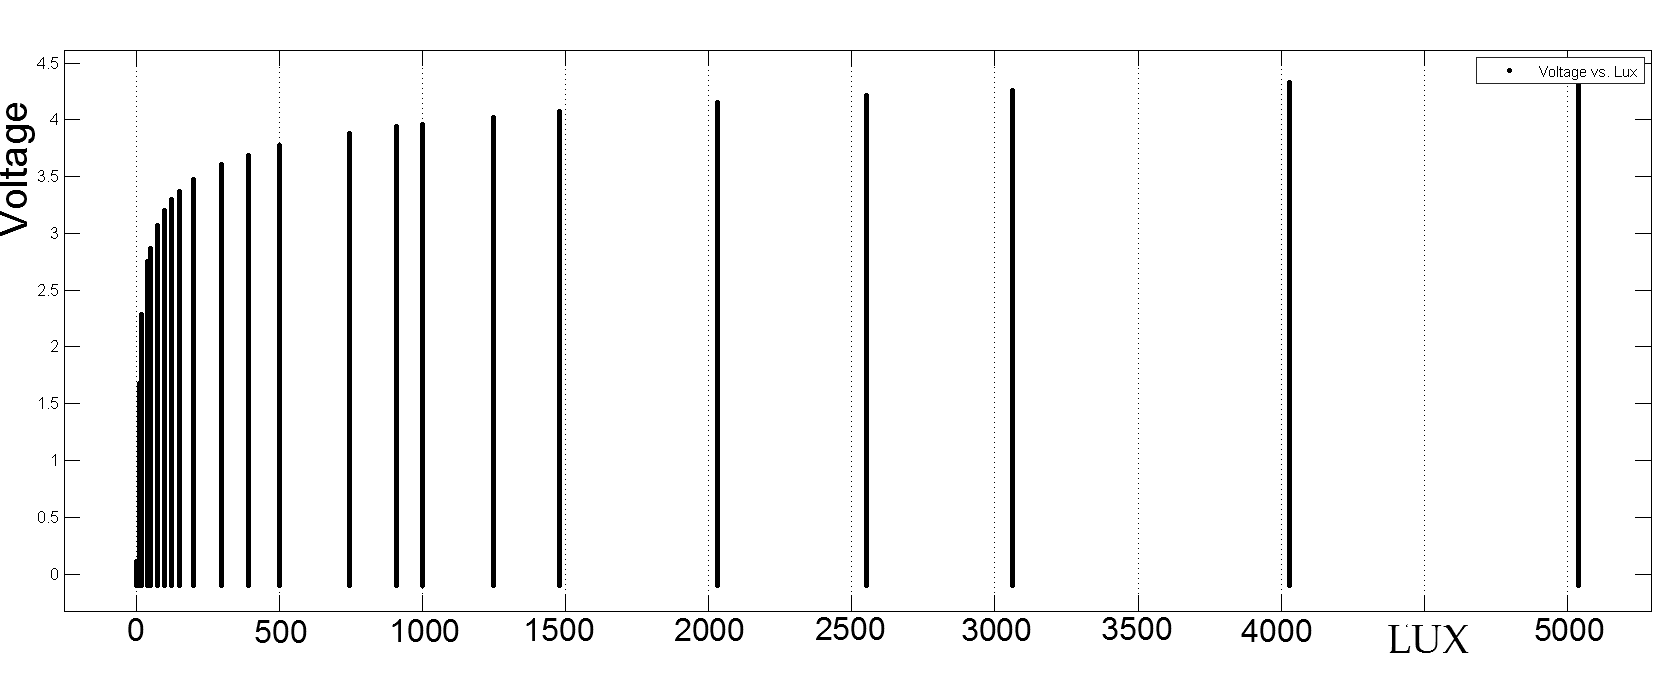
\includegraphics[width=0.9\linewidth]{images/Voltagevlux}
	\caption{spread of measured illumination vs Voltage  }
	\label{fig:Voltagevlux}
  \end{center}
 \end{figure}
 The Cell-under-test is connected to a \ac{SMU}. \ac{SMU}s have flexibility in their outputs, to be classified as having four-quadrant outputs, it must be able to source power as well as sink power. Sourcing power refers to providing the stimulus for a circuit, and sinking power refers to dissipating power that is being applied by an external active component such as a battery, a charged capacitor, or another power source \cite{NI_SMU} - a solar cell in our case.
 \begin{figure}[H]
	  \begin{center}
		  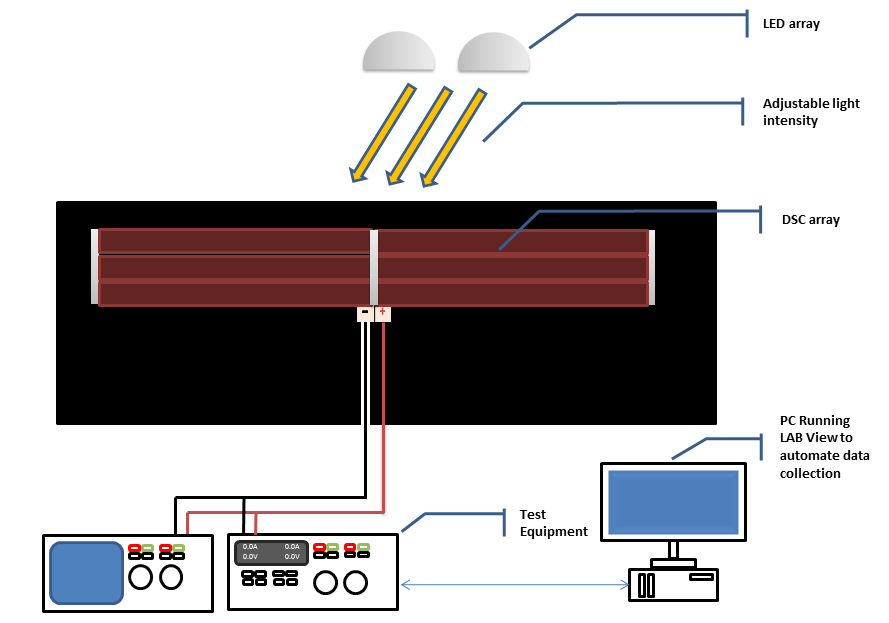
\includegraphics[width=\textwidth]{images/Cell_under_test}
		  \caption{Cell Characterisation }
		  \label{fig:Cell_U_test}
	  \end{center}
 \end{figure}
 As the Sink potential is increased in tiny increments, starting from  0 V to V\textsubscript{OC} and beyond, the cell is forced to operate at the Sink Voltage resulting in the I-V graph depicted in figure ~\ref{fig:2500luxIV} on page ~\pageref{fig:2500luxIV}. When the above is repeated for several different light intensities we get a three-dimensional surface shown in figure ~\ref{fig:luxIV100_2500} on page ~\pageref{fig:luxIV100_2500}.Note that, V\textsubscript{OC} is the maximum voltage available from a cell this occurs when the cell produces zero Current (when the graph intersects the \textit{x}-axis).\\
 
  \begin{figure}[H]
	  \begin{center}
		  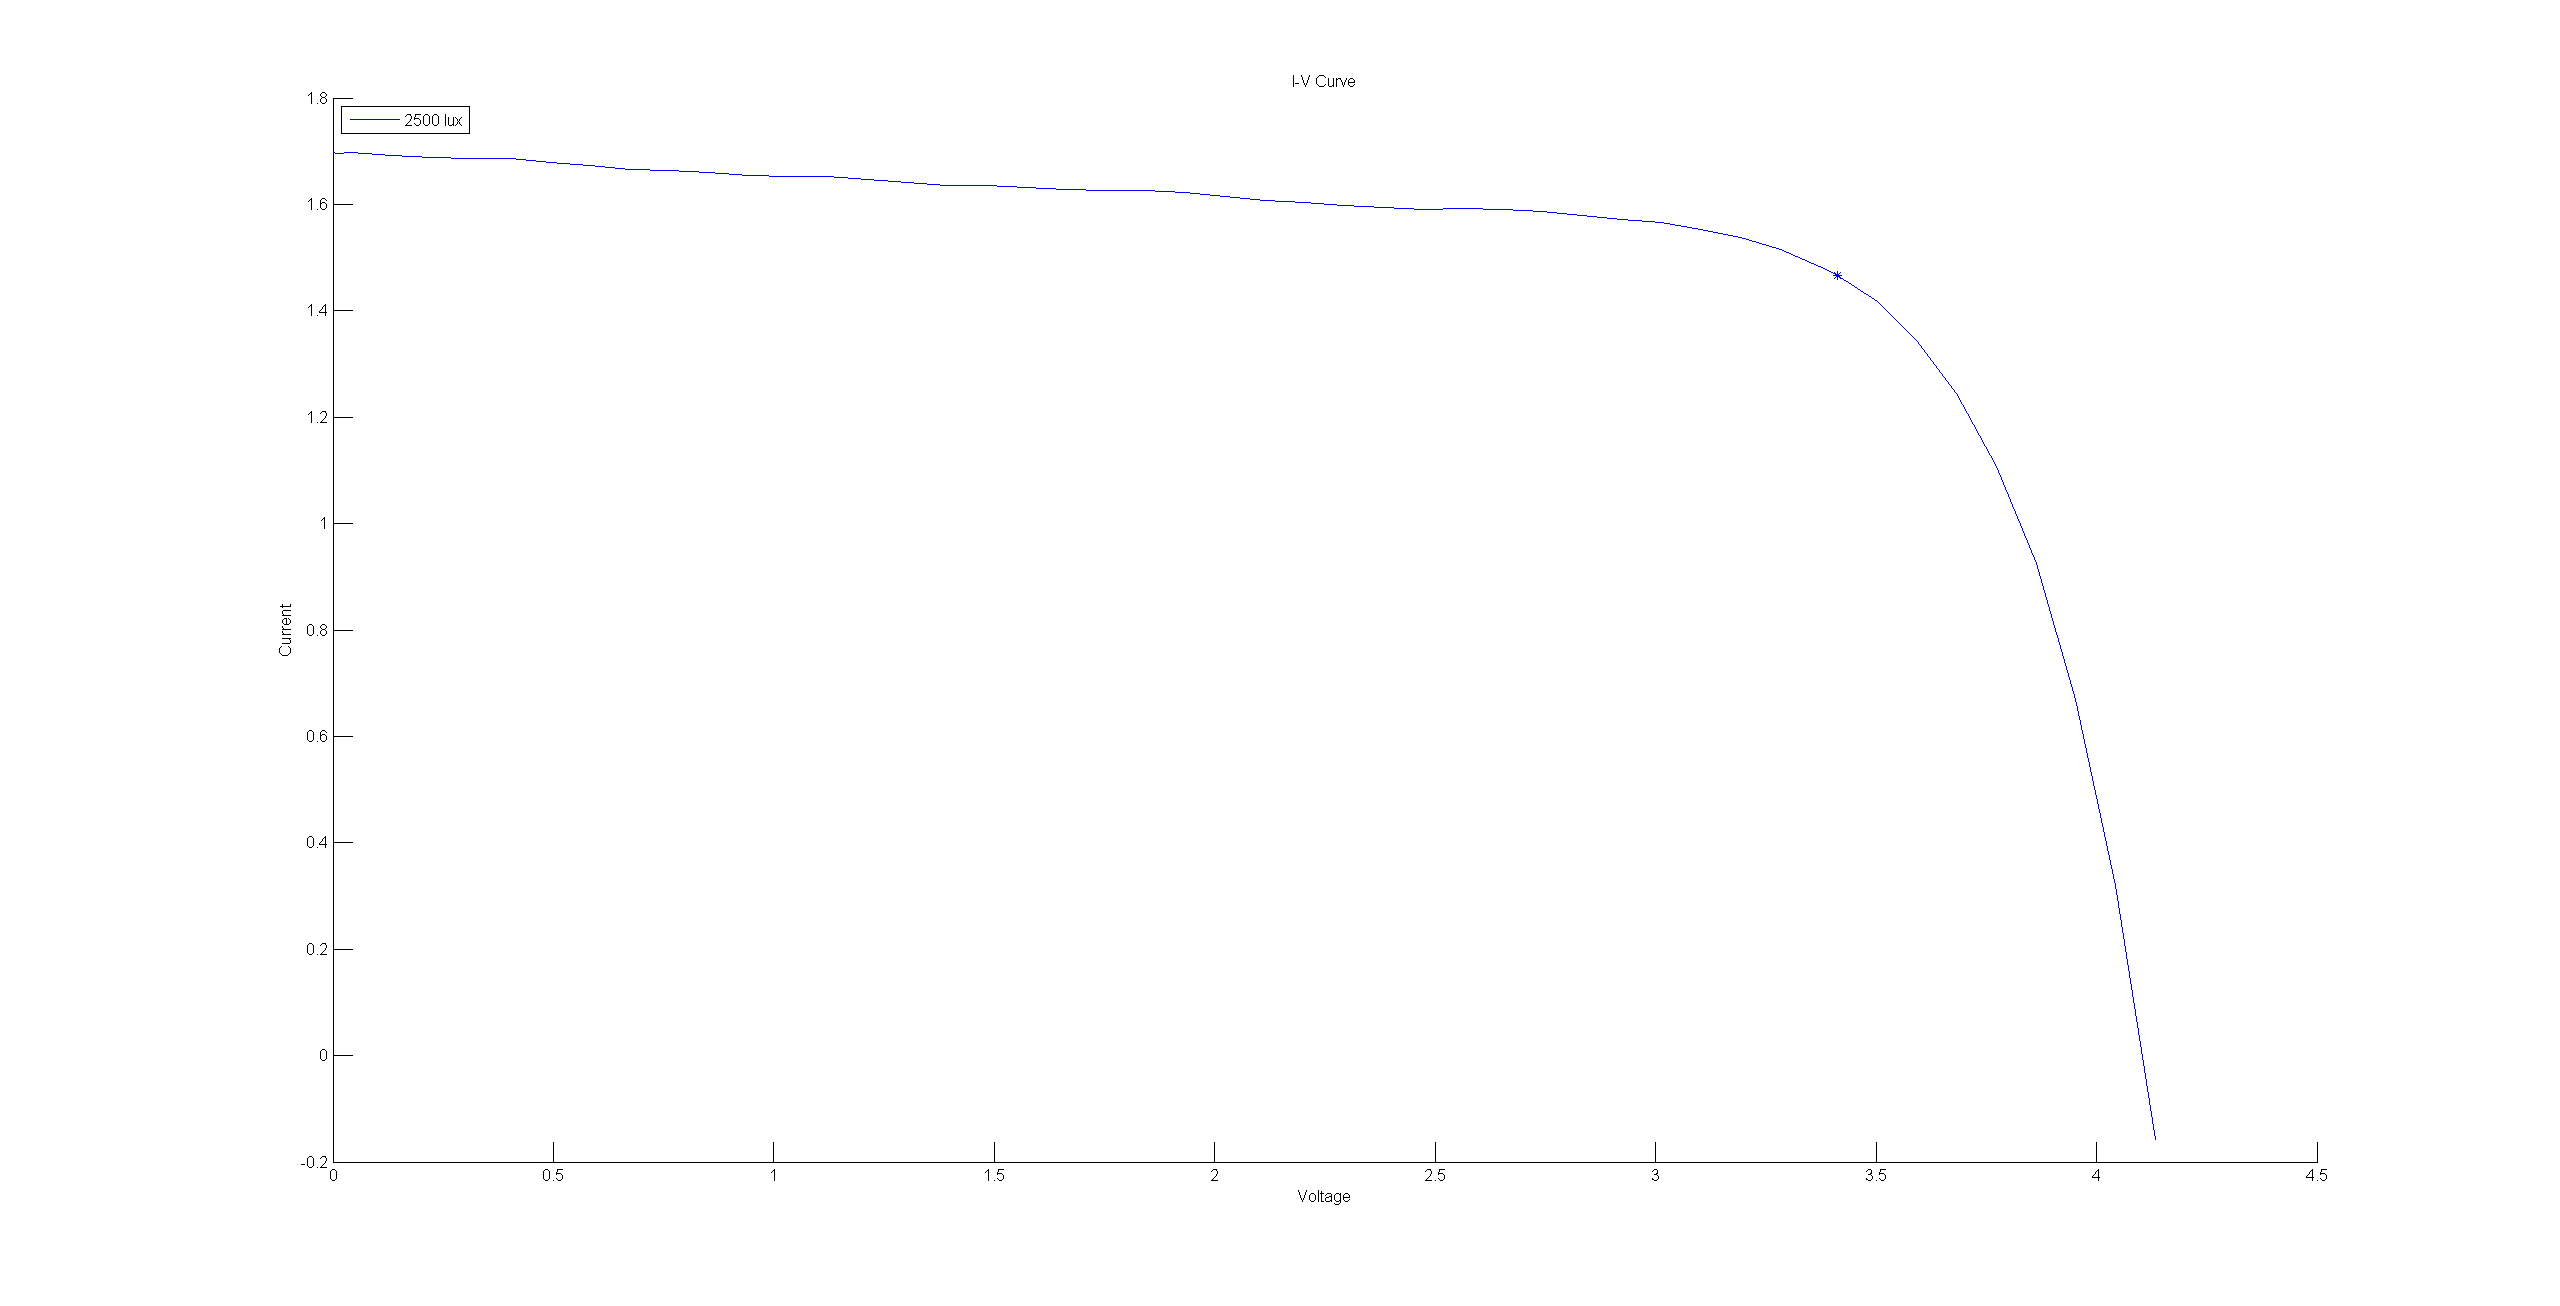
\includegraphics[width=1.1\textwidth]{images/single2500_IV}
		  \caption{I-V curve for the array at steady illumination}
		  \label{fig:2500luxIV}
	  \end{center}
  \end{figure}
  
\begin{figure}[H]
	  \begin{center}
		  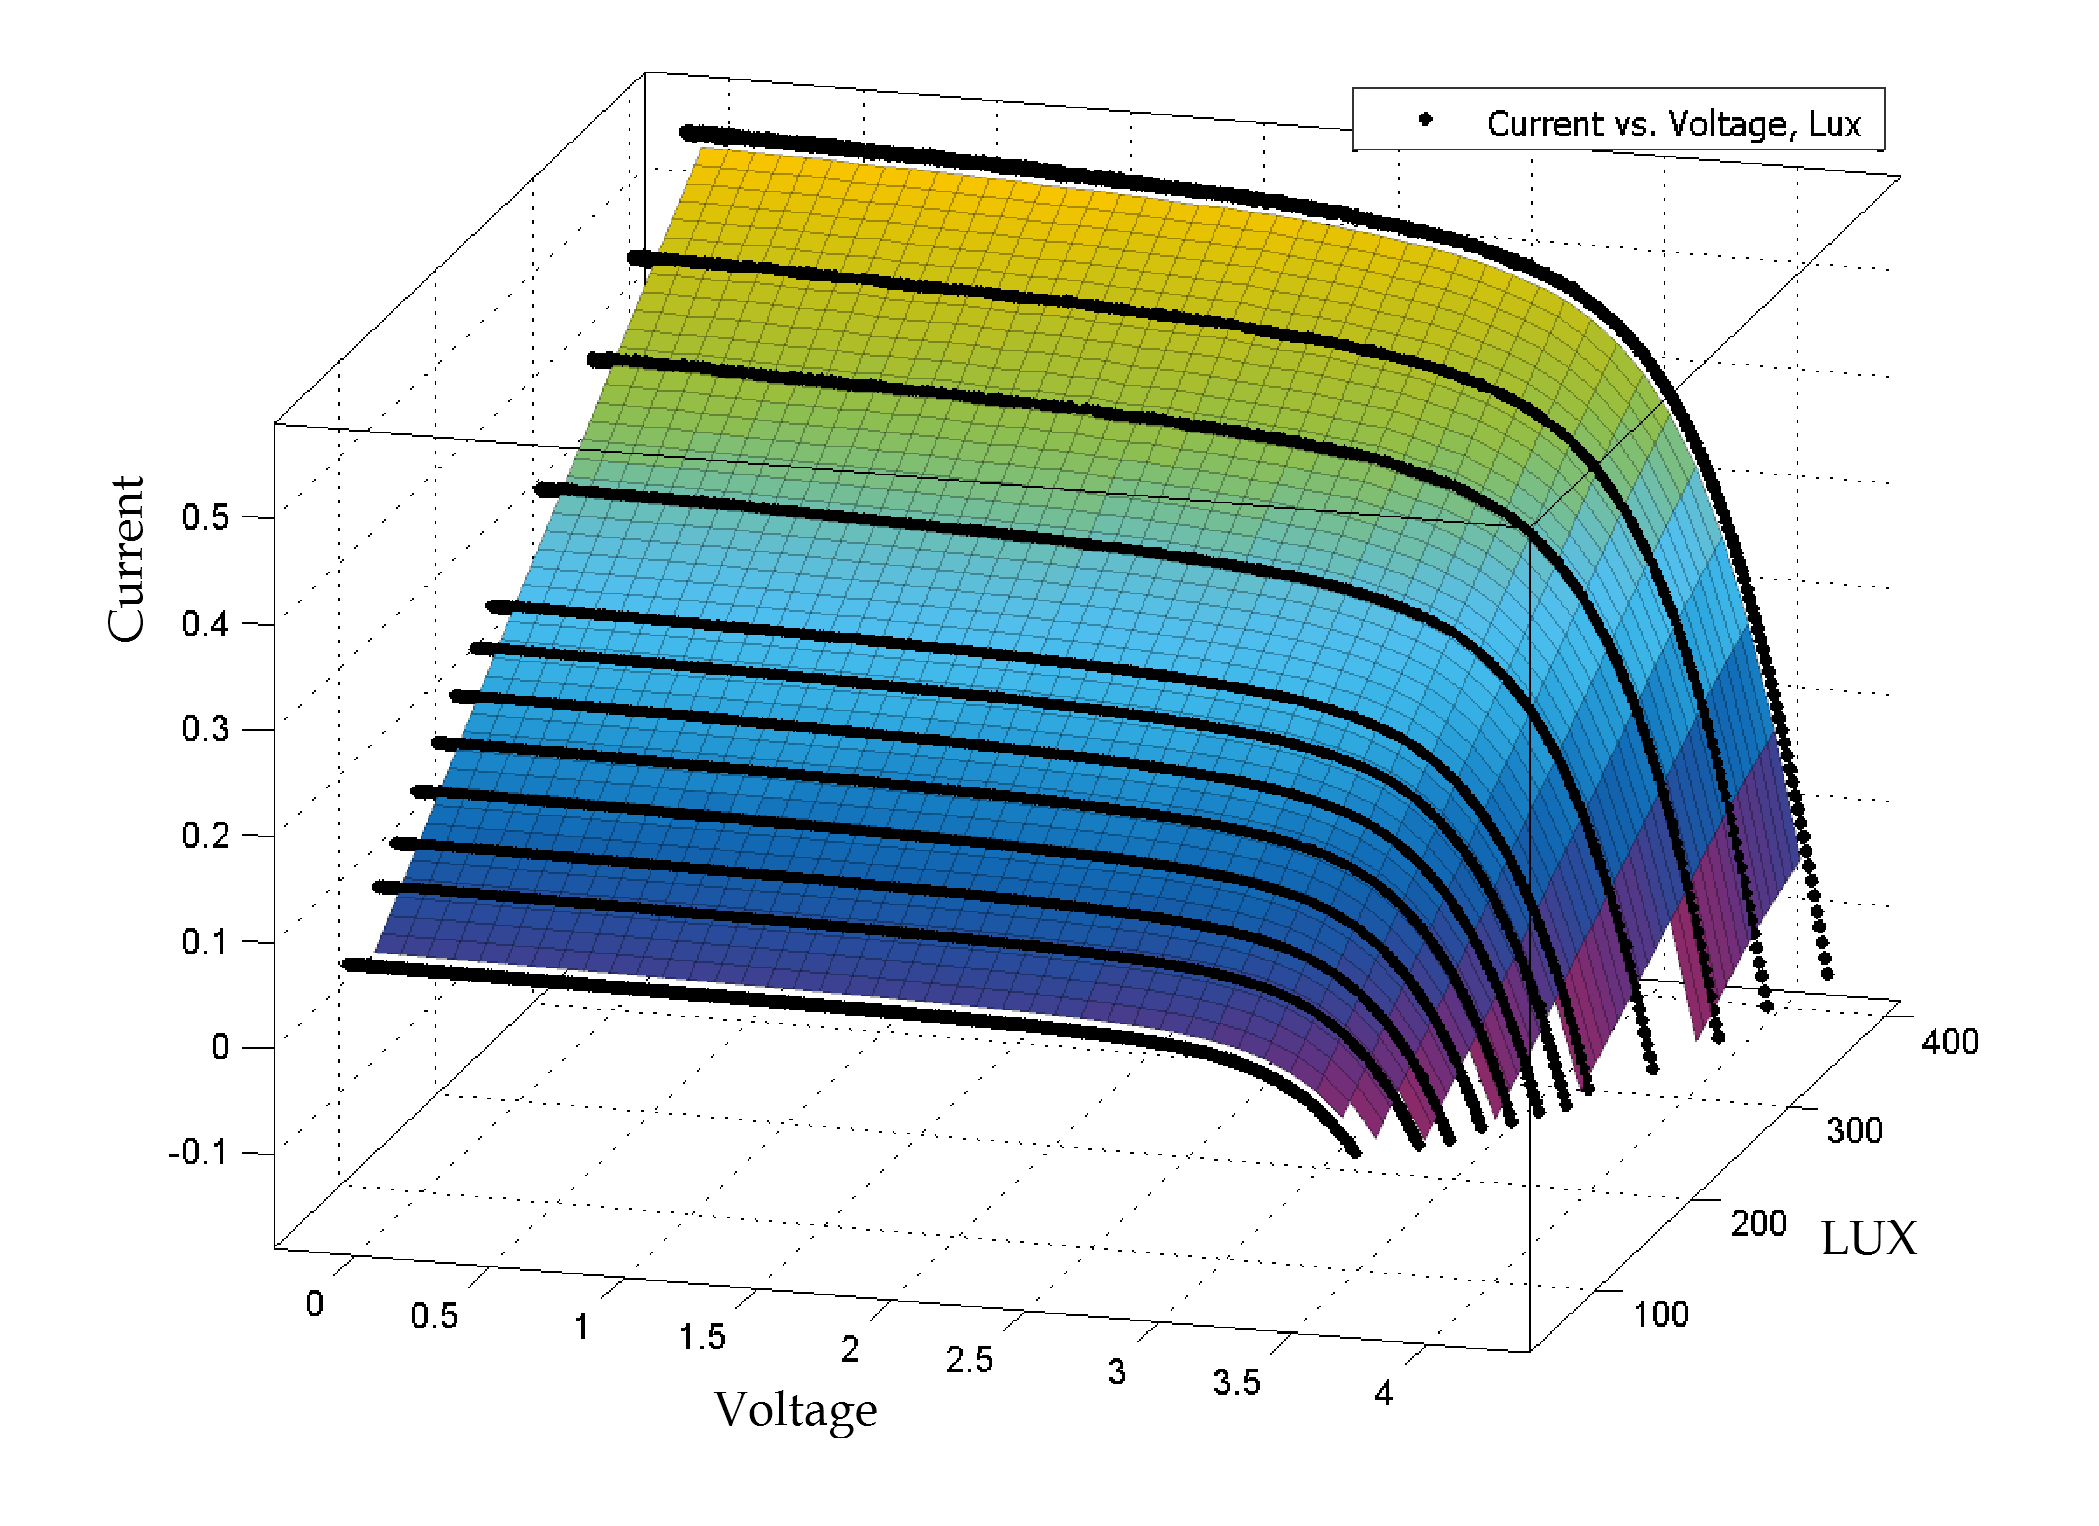
\includegraphics[width=0.8\textwidth]{images/I-V-lux}
		  \caption{I-V curve for the array at varying illumination}
		  \label{fig:luxIV100_2500}
	  \end{center}
  \end{figure}

\section{Modelling and Simulations} 

The three-dimensional surface thus created in the section above acts as a function, a look-up table of sorts, for a given illumination and voltage; the function computes a appropriate value for the cell's current . ** to convert continuous voltage values to discreet values **,a transfer functions are used. The \ac{DSCs} subsystem is represented in the figure ~\ref{fig:PV_block_Model} below. Capacitor is added in order to accurately mimic the response of \ac{DSCs} under test as discussed in \ref{sec:eDDM}. The diode acts as a Snubber, eliminating flyback across the inductive load. This sub-system is placed under a mask in the abstract view, shown in figure ~\ref{fig:Model_top} on page ~\pageref{fig:Model_top}, in order to simplify operation and for ascetic reasons. The validation of the said model is discussed in section \ref{sec:Validation}. Another look-up table provides Open-circuit Voltages ($V_{OC}$) for a given Lux, to be used in certain algorithms. \\

The \textit{Scopes and Outputs} subsection is used to plot data on to graphs and to push data onto Matlab, for further analysis.\\

The \ac{MPPT} \textit{Controller Block} (figure ~\ref{fig:Controller_mod} on page ~\pageref{fig:Controller_mod} ) is modelled as a variant subsystem. The variant-control determines which variant is active, and is set before the simulation is started. This arrangement of subsystems makes it extremely easy to switch between and compare the various \ac{MPPT} Algorithms without making any alterations to the rest of the model.    

\begin{figure}[H]
	  \begin{center}
		  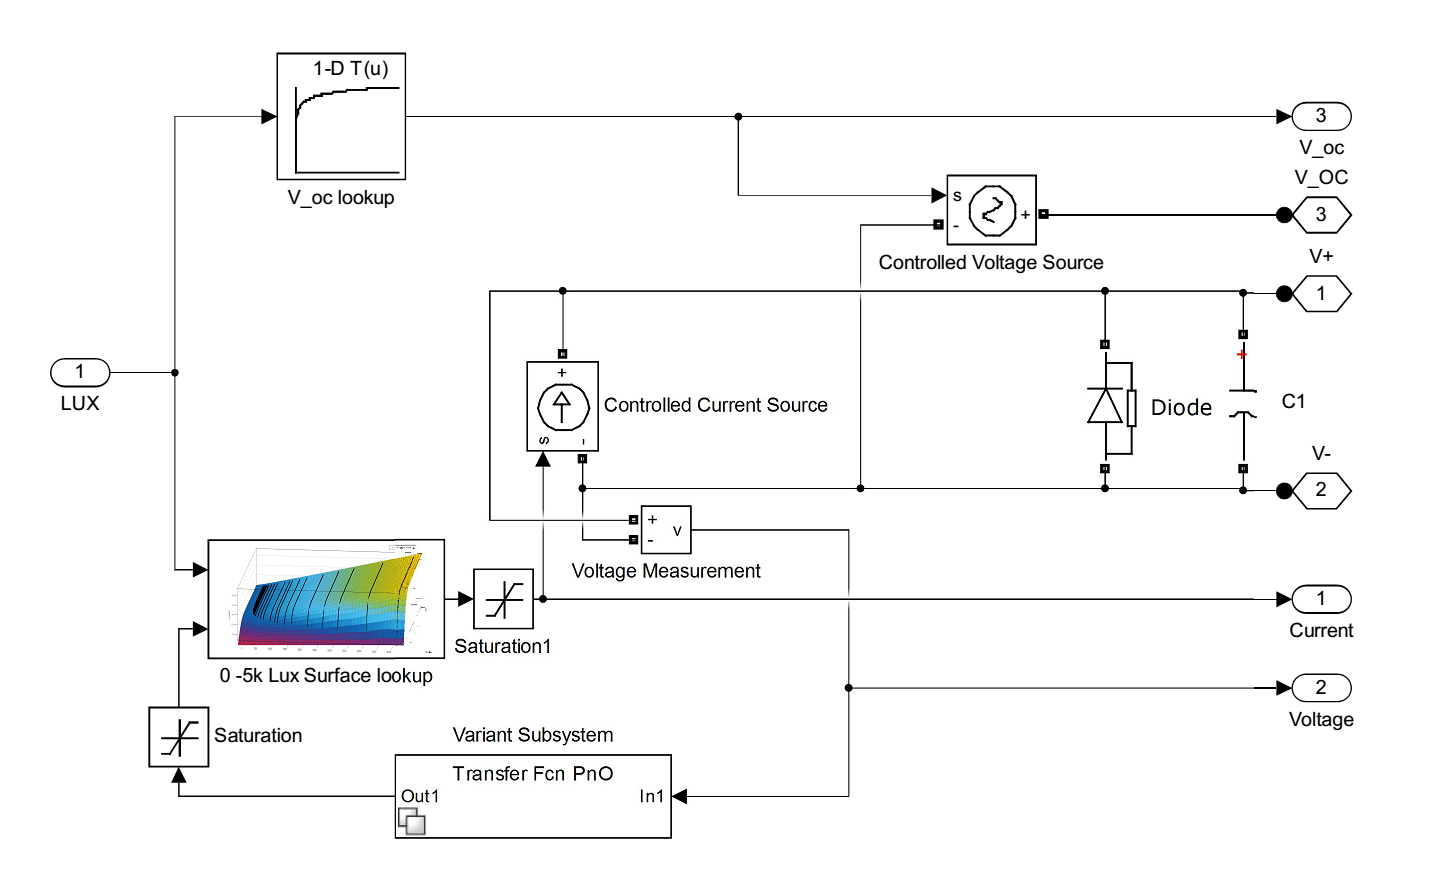
\includegraphics[width=\textwidth]{images/PV_block_Model}
		  \caption{Modelling of the DSC Subsystem }
		  \label{fig:PV_block_Model}
	  \end{center}
  \end{figure}

\begin{figure}[H]
  \begin{center}
	  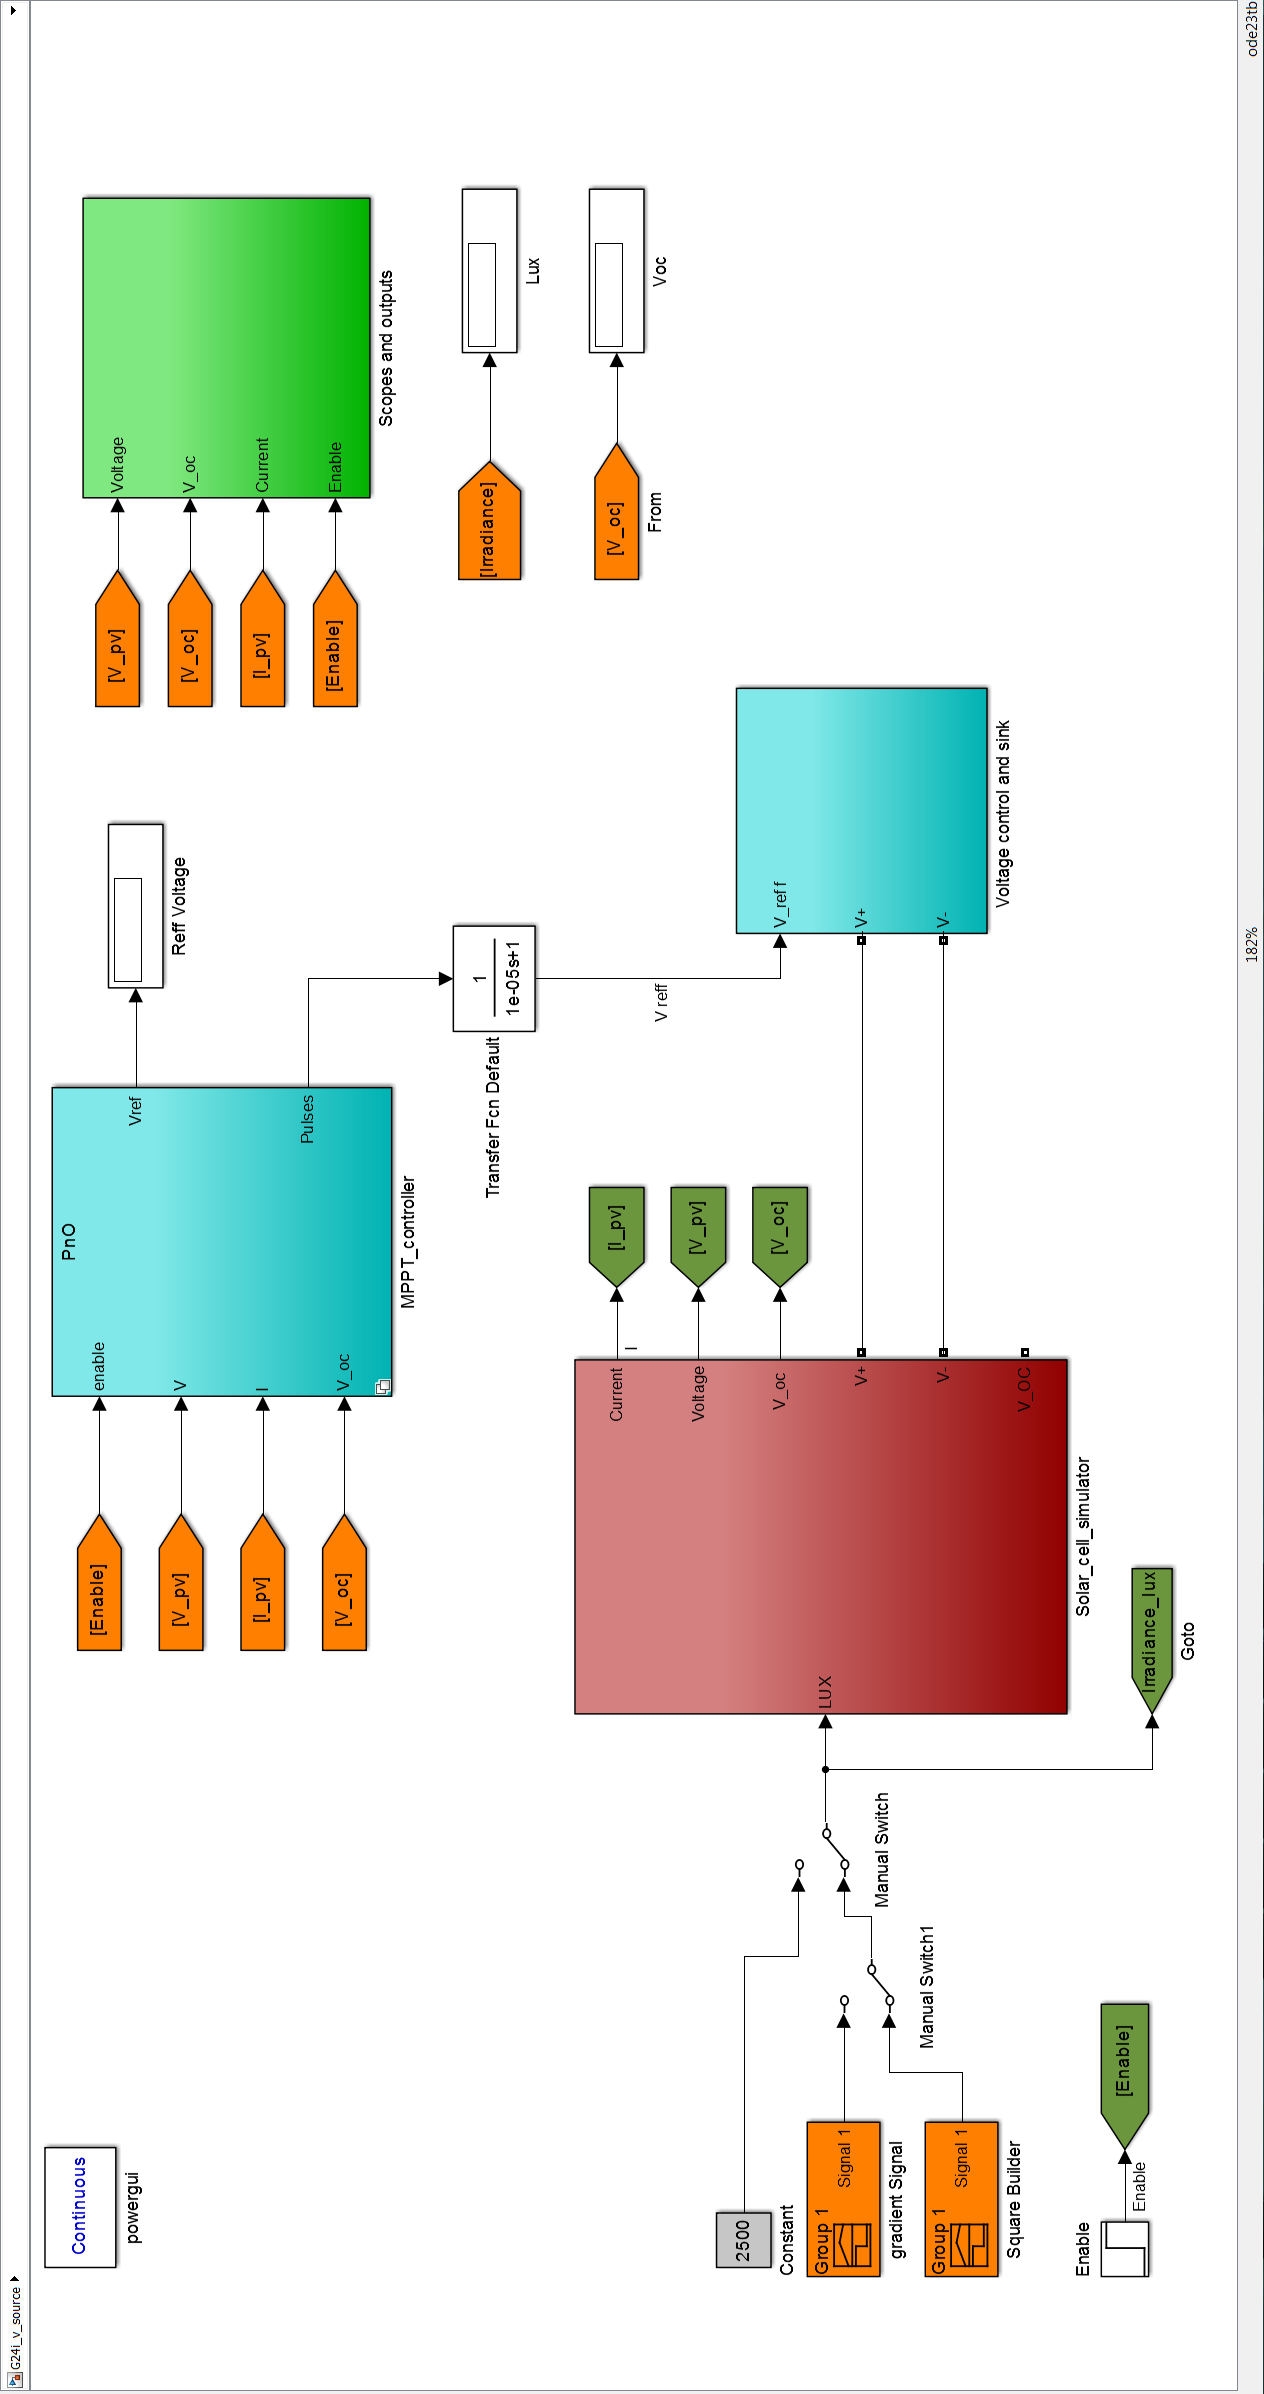
\includegraphics[width=\textwidth]{images/Top_level_mod}
	  \caption{Top Model }
	  \label{fig:Model_top}
  \end{center}
\end{figure}

\begin{figure}[H]
  \begin{center}
	  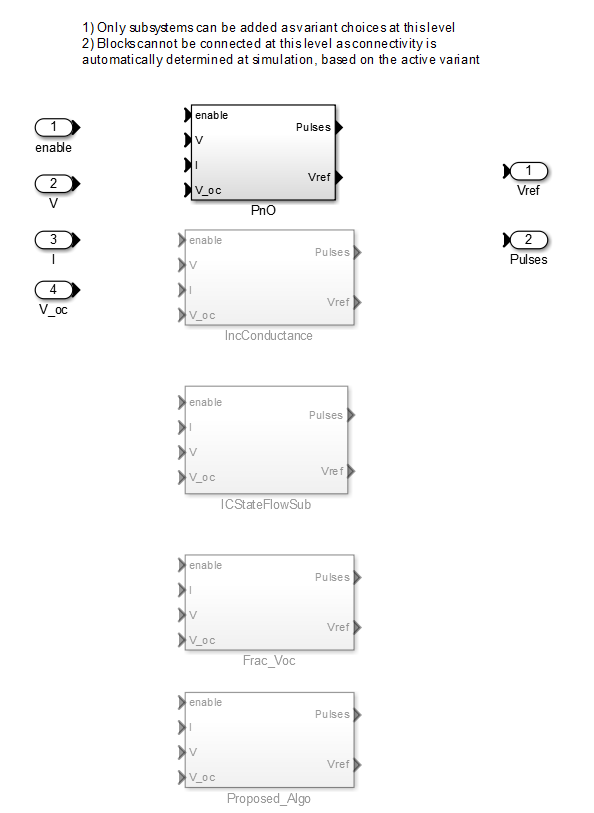
\includegraphics[width=0.9\textwidth]{images/controller_mod}
	  \caption{MPPT controller }
	  \label{fig:Controller_mod}
  \end{center}
\end{figure}
 



\section {Validation of the model in Matlab{\textregistered}}\label{sec:Validation} 

Since the credibility of the thesis rests on the accuracy of the model used to compare the different algorithms, therefore a section is devoted to the validation of the same. \ref{sec:cel_char}


\begin{figure}[H]
	  \begin{center}
		  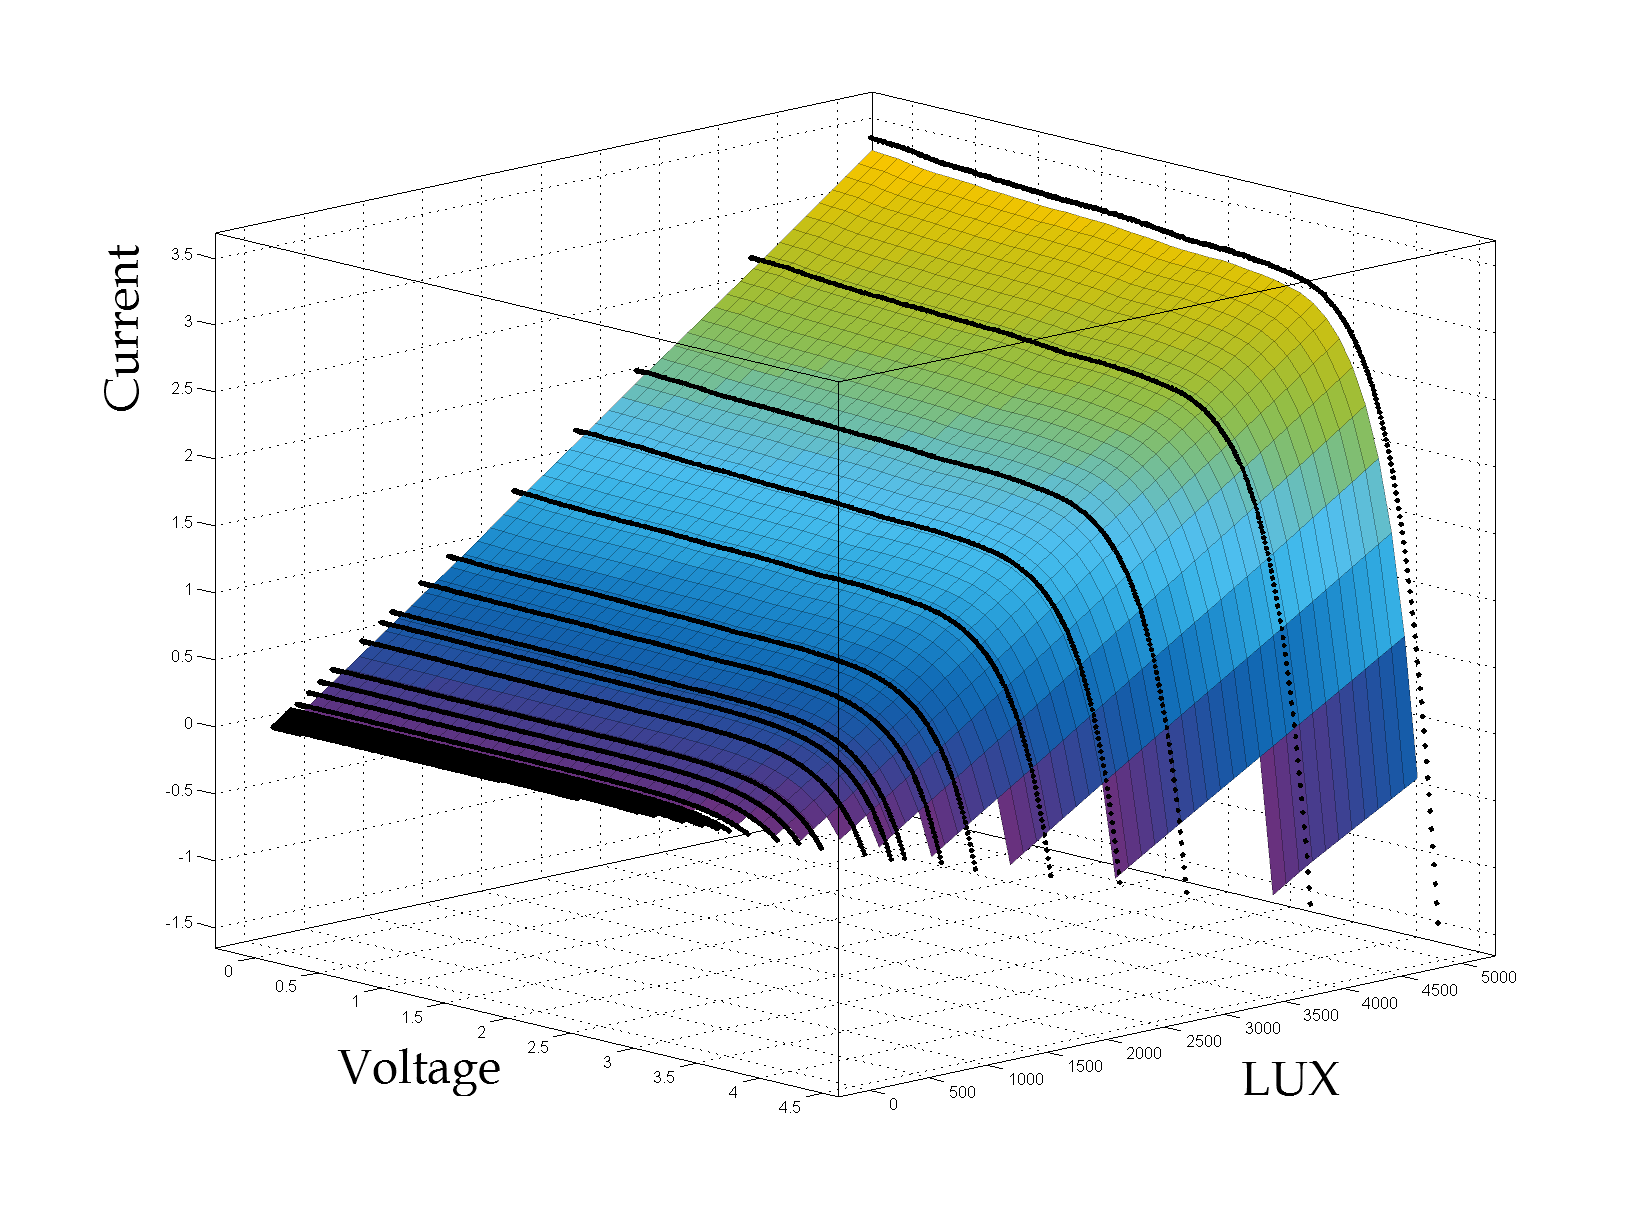
\includegraphics[width=0.8\textwidth]{images/IVLUX_LAB_measured}
		  \caption{3-D representation of the cell's characteristics measured in the lab }
		  \label{fig:IVLUX_LAB_measured}
	  \end{center}
  \end{figure}

\begin{figure}[H]
  \begin{center}
	  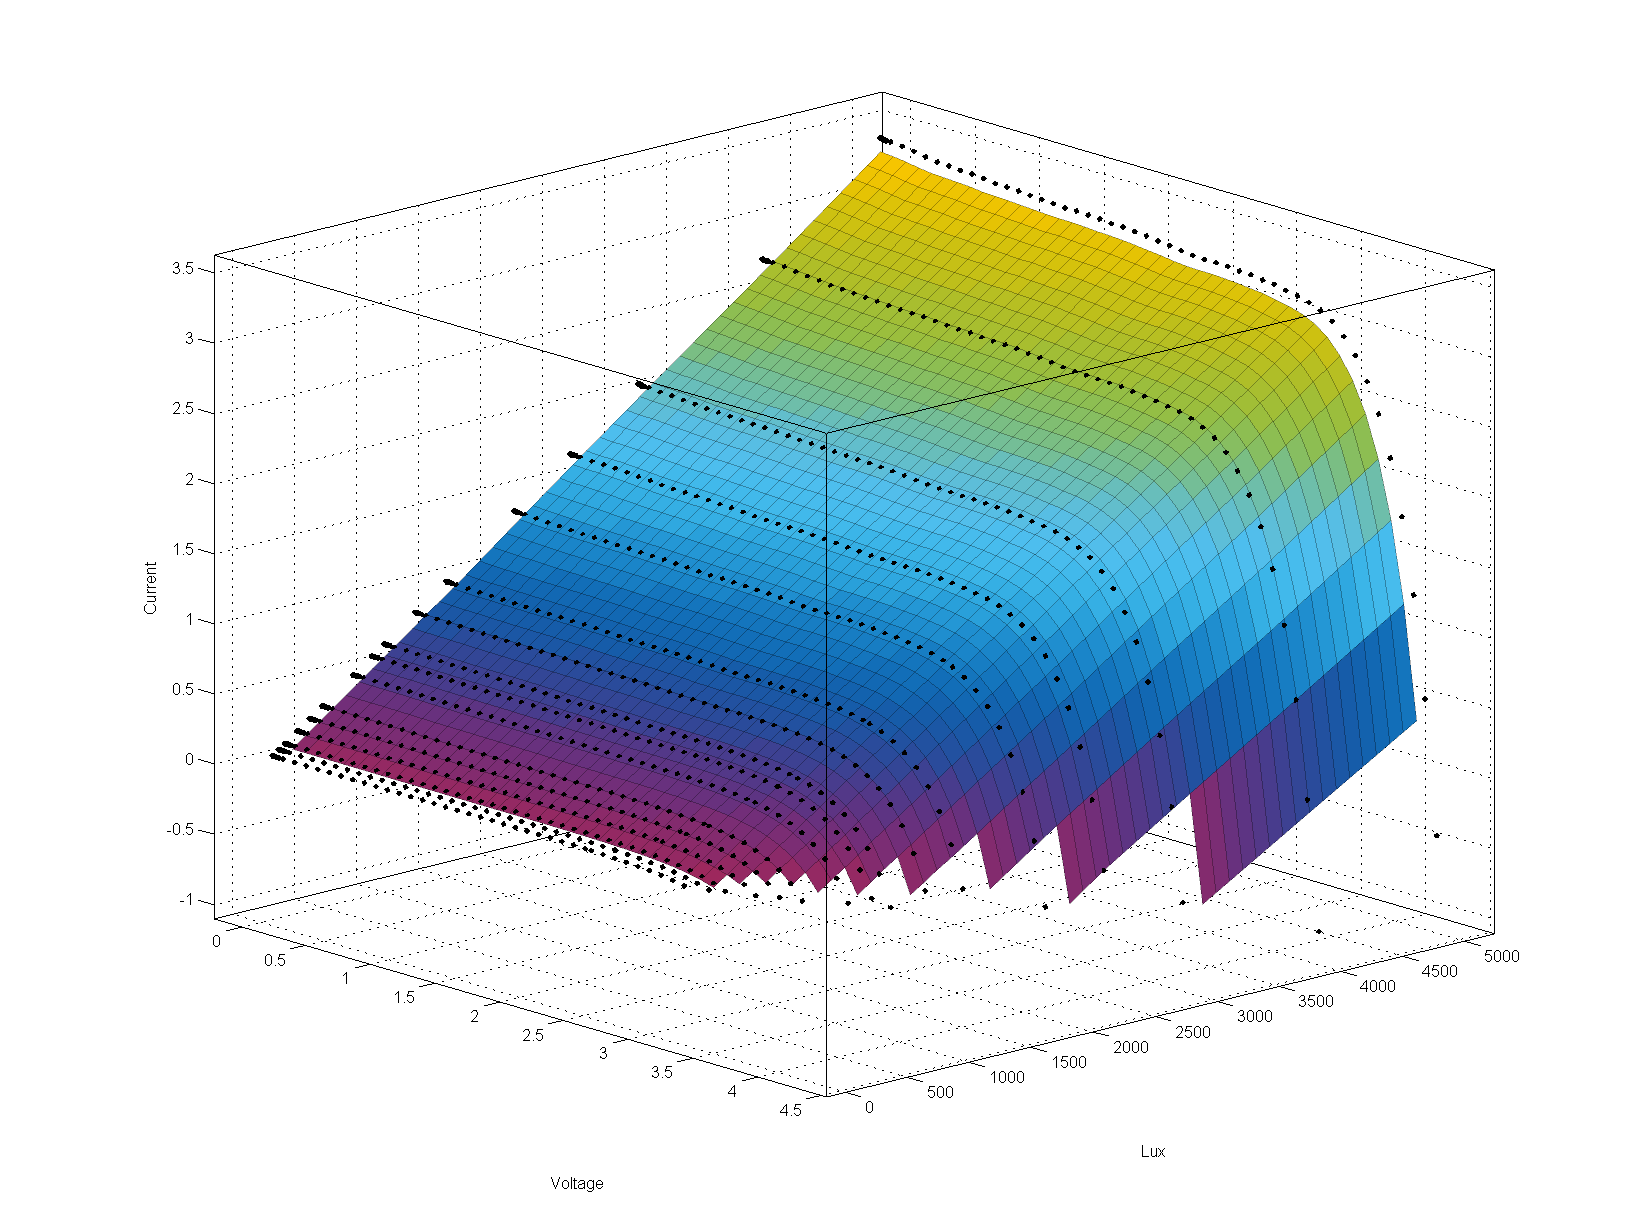
\includegraphics[width=0.8\textwidth]{images/IVLUX_MOD_gen}
	  \caption{Surface generated by the Matlab model}
	  \label{fig:IVLUX_MOD_gen}
  \end{center}
\end{figure}

\begin{figure}[H]
  \begin{center}
	  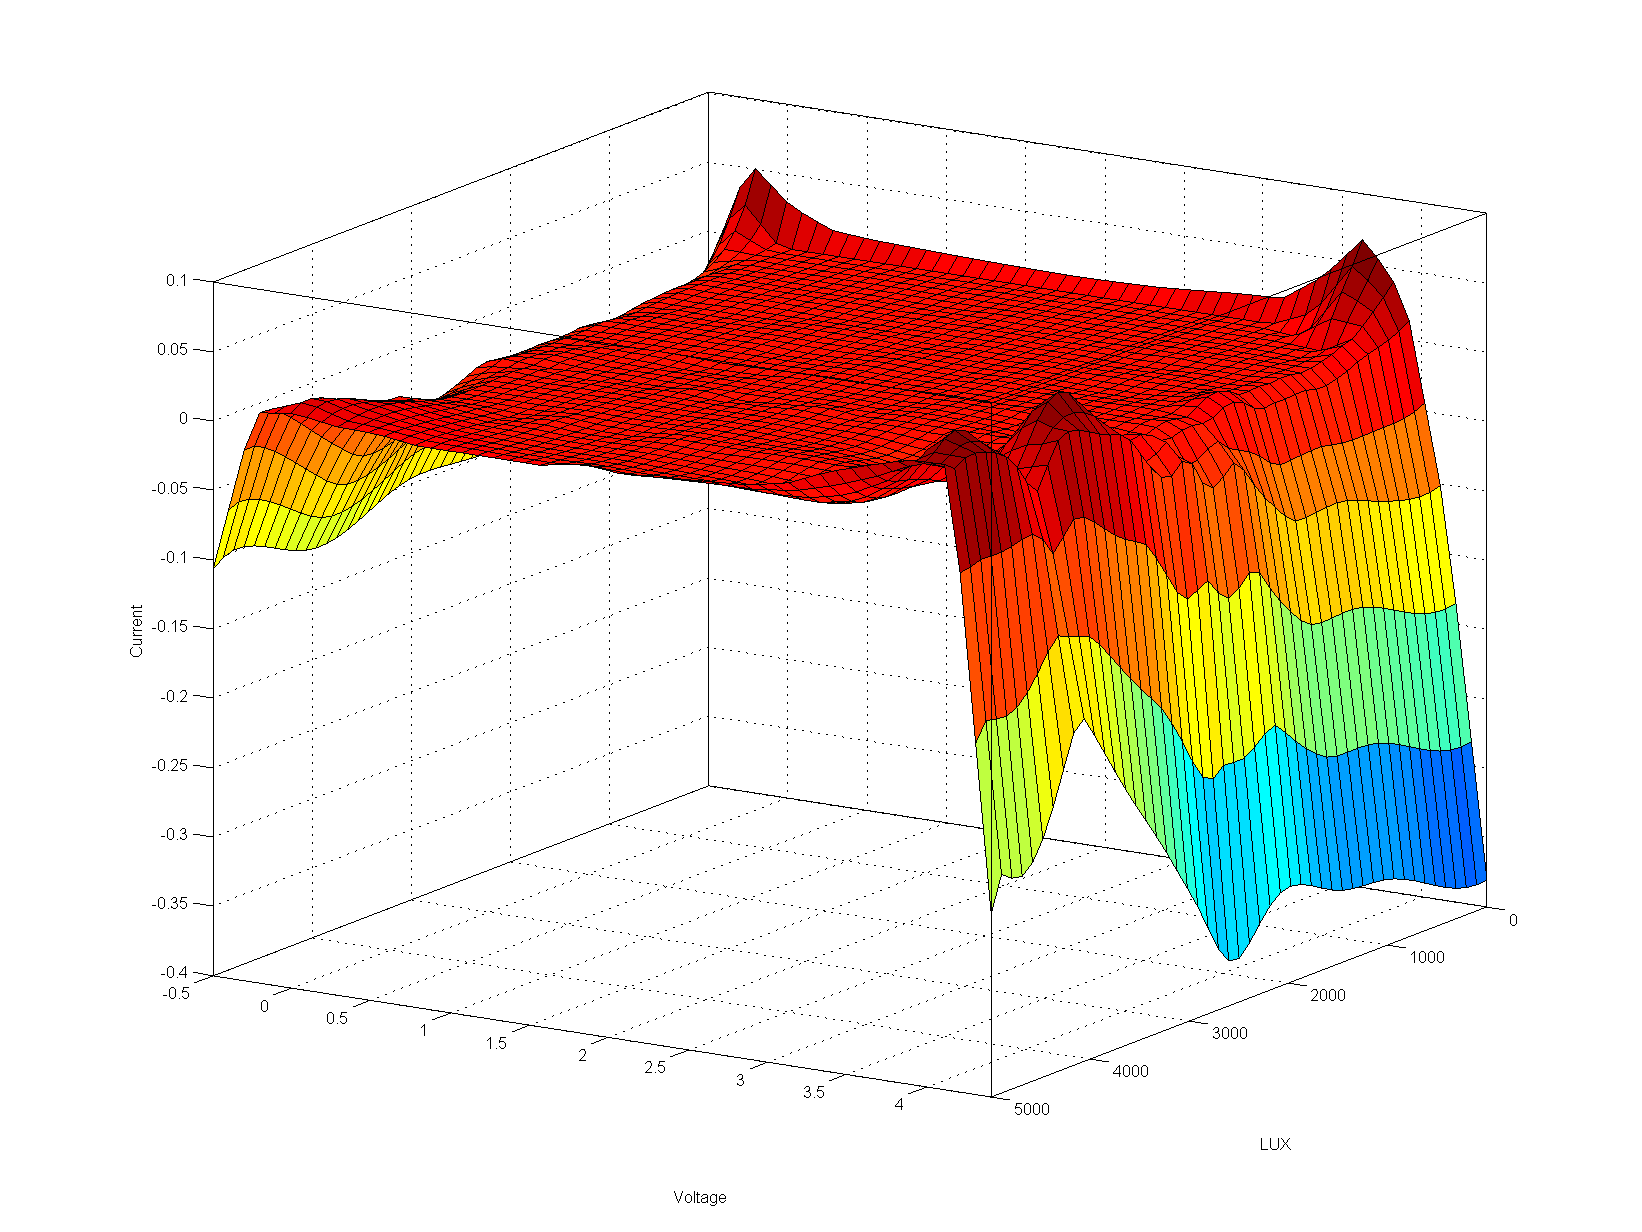
\includegraphics[width=\textwidth]{images/Diff_Contour}
	  \caption{Model resulting from the difference of the two models (Figures ~\ref{fig:IVLUX_LAB_measured} \&~\ref{fig:IVLUX_MOD_gen} )  }
	  \label{fig:Diff_Contour}
  \end{center}
\end{figure}

\begin{figure}[H]
  \begin{center}
	  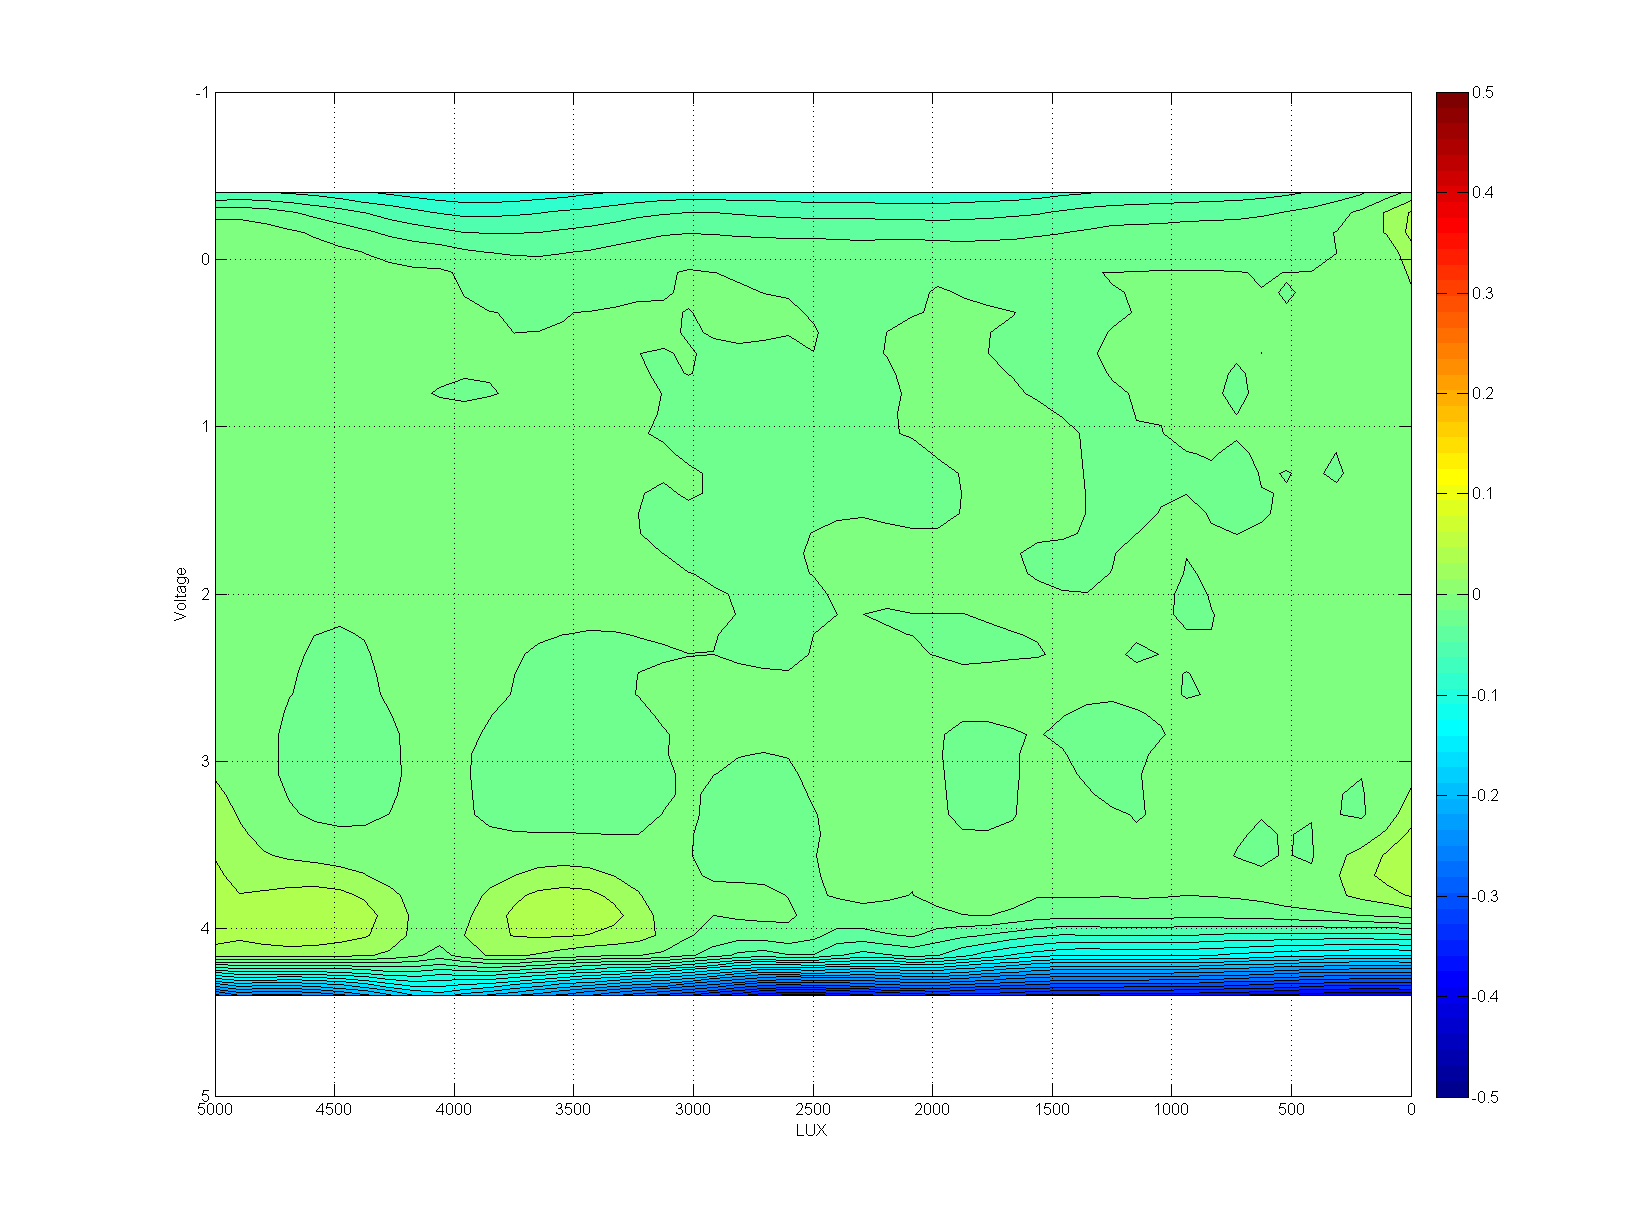
\includegraphics[width=\textwidth]{images/Contour_map}
	  \caption{Contour map of the difference}
	  \label{fig:Contour_map}
  \end{center}
\end{figure}

\section{Proposed Method }

\cite{houssamo2013experimental}

This work presents an experimental comparison; Using four identical PV, under strictly the same set of technical and meteorological conditions, an experimental comparison  of four most used MPPT methods for PV power systems is done.This comparison shows the advantage of use of a MPPT with a variable tracking step.\\  

\cite{jain2004new}
This paper presents a new algorithm for tracking maximum power point in photovoltaic systems. This is a fast tracking algorithm, where an initial approximation of \ac{MPP} quickly achieved using a variable step-size. Subsequently, the exact\ac{MPP} can be targeted using any conventional method like the hill-climbing or incremental conductance method. Thus, the drawback of a fixed small step-size over the entire tracking range is removed, resulting in reduced number of iterations and much faster tracking compared to conventional methods. \\
 My implementation draws inspiration for the above article for its  two-stage algorithm to reduce the number of iterations but deviates significantly in the implementation and algorithms used to identify the \ac{MPP} 
 
\cite{liu2011fast}

\begin{figure}[H]
  \begin{center}
	  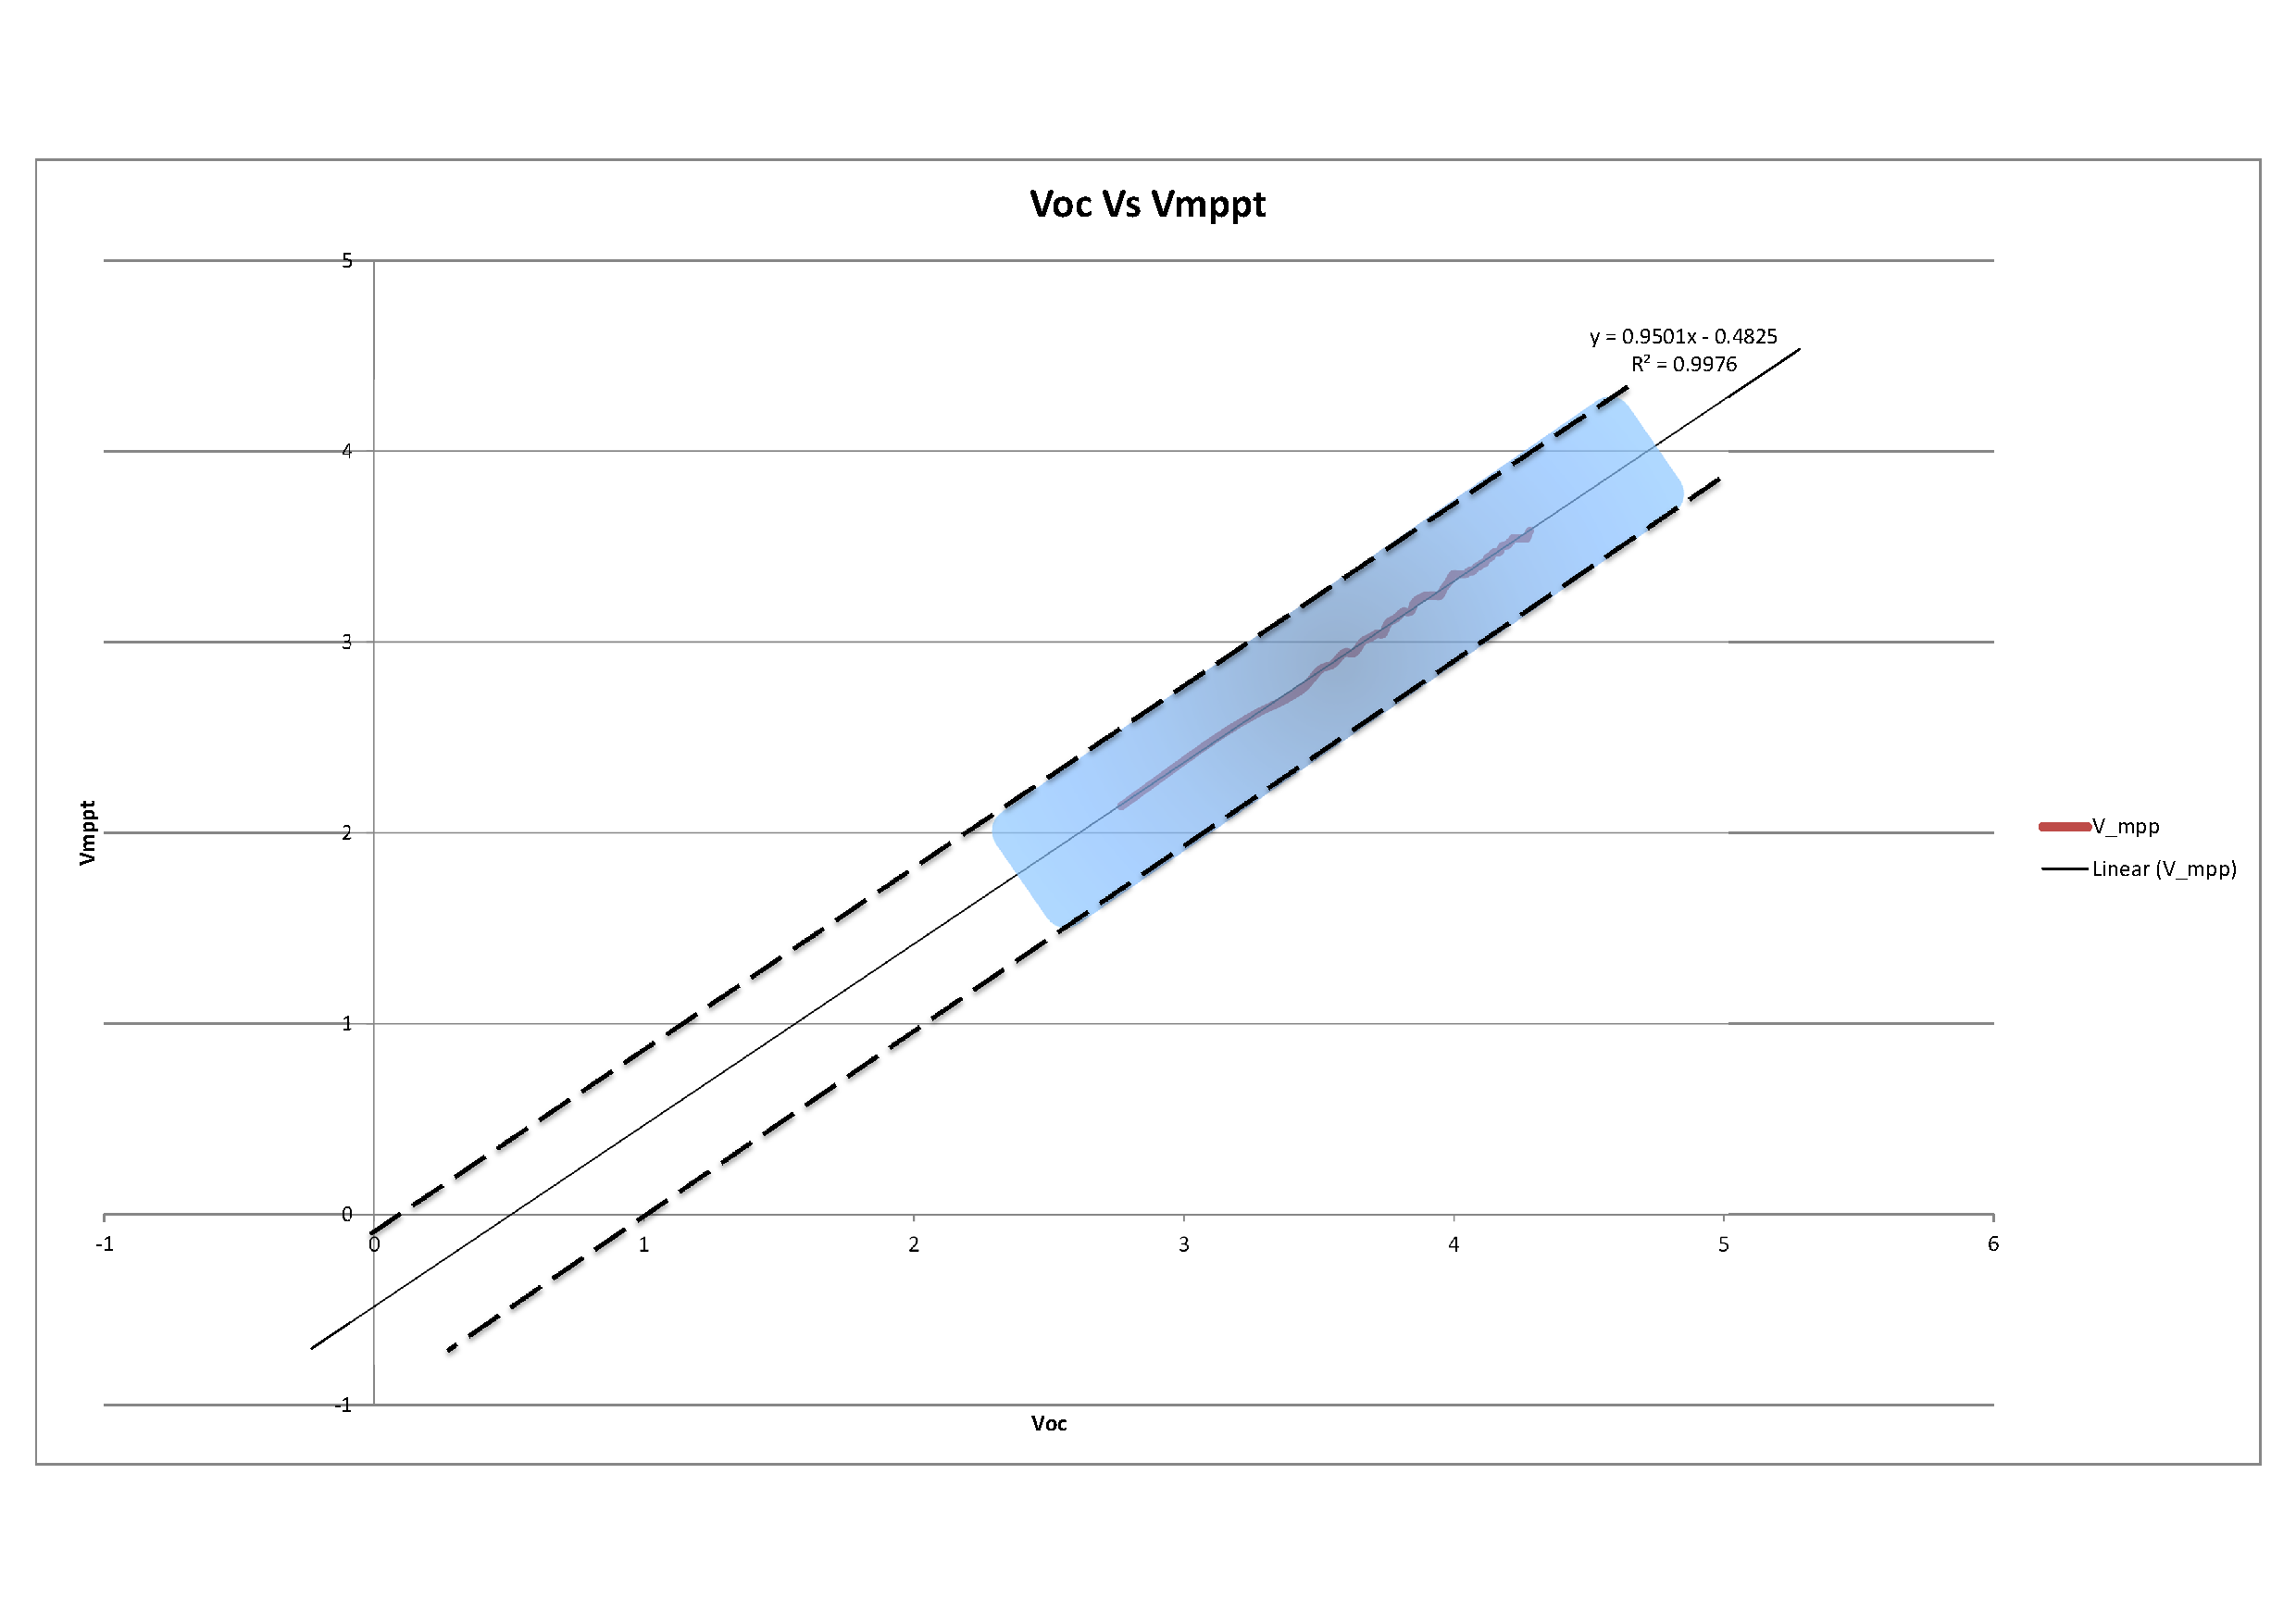
\includegraphics[width=1.1\textwidth]{images/Probability_field}
	  \caption{Probability field }
	  \label{fig:Probability_field}
  \end{center}
\end{figure}

  \begin{figure}[H]
    \begin{center}
	   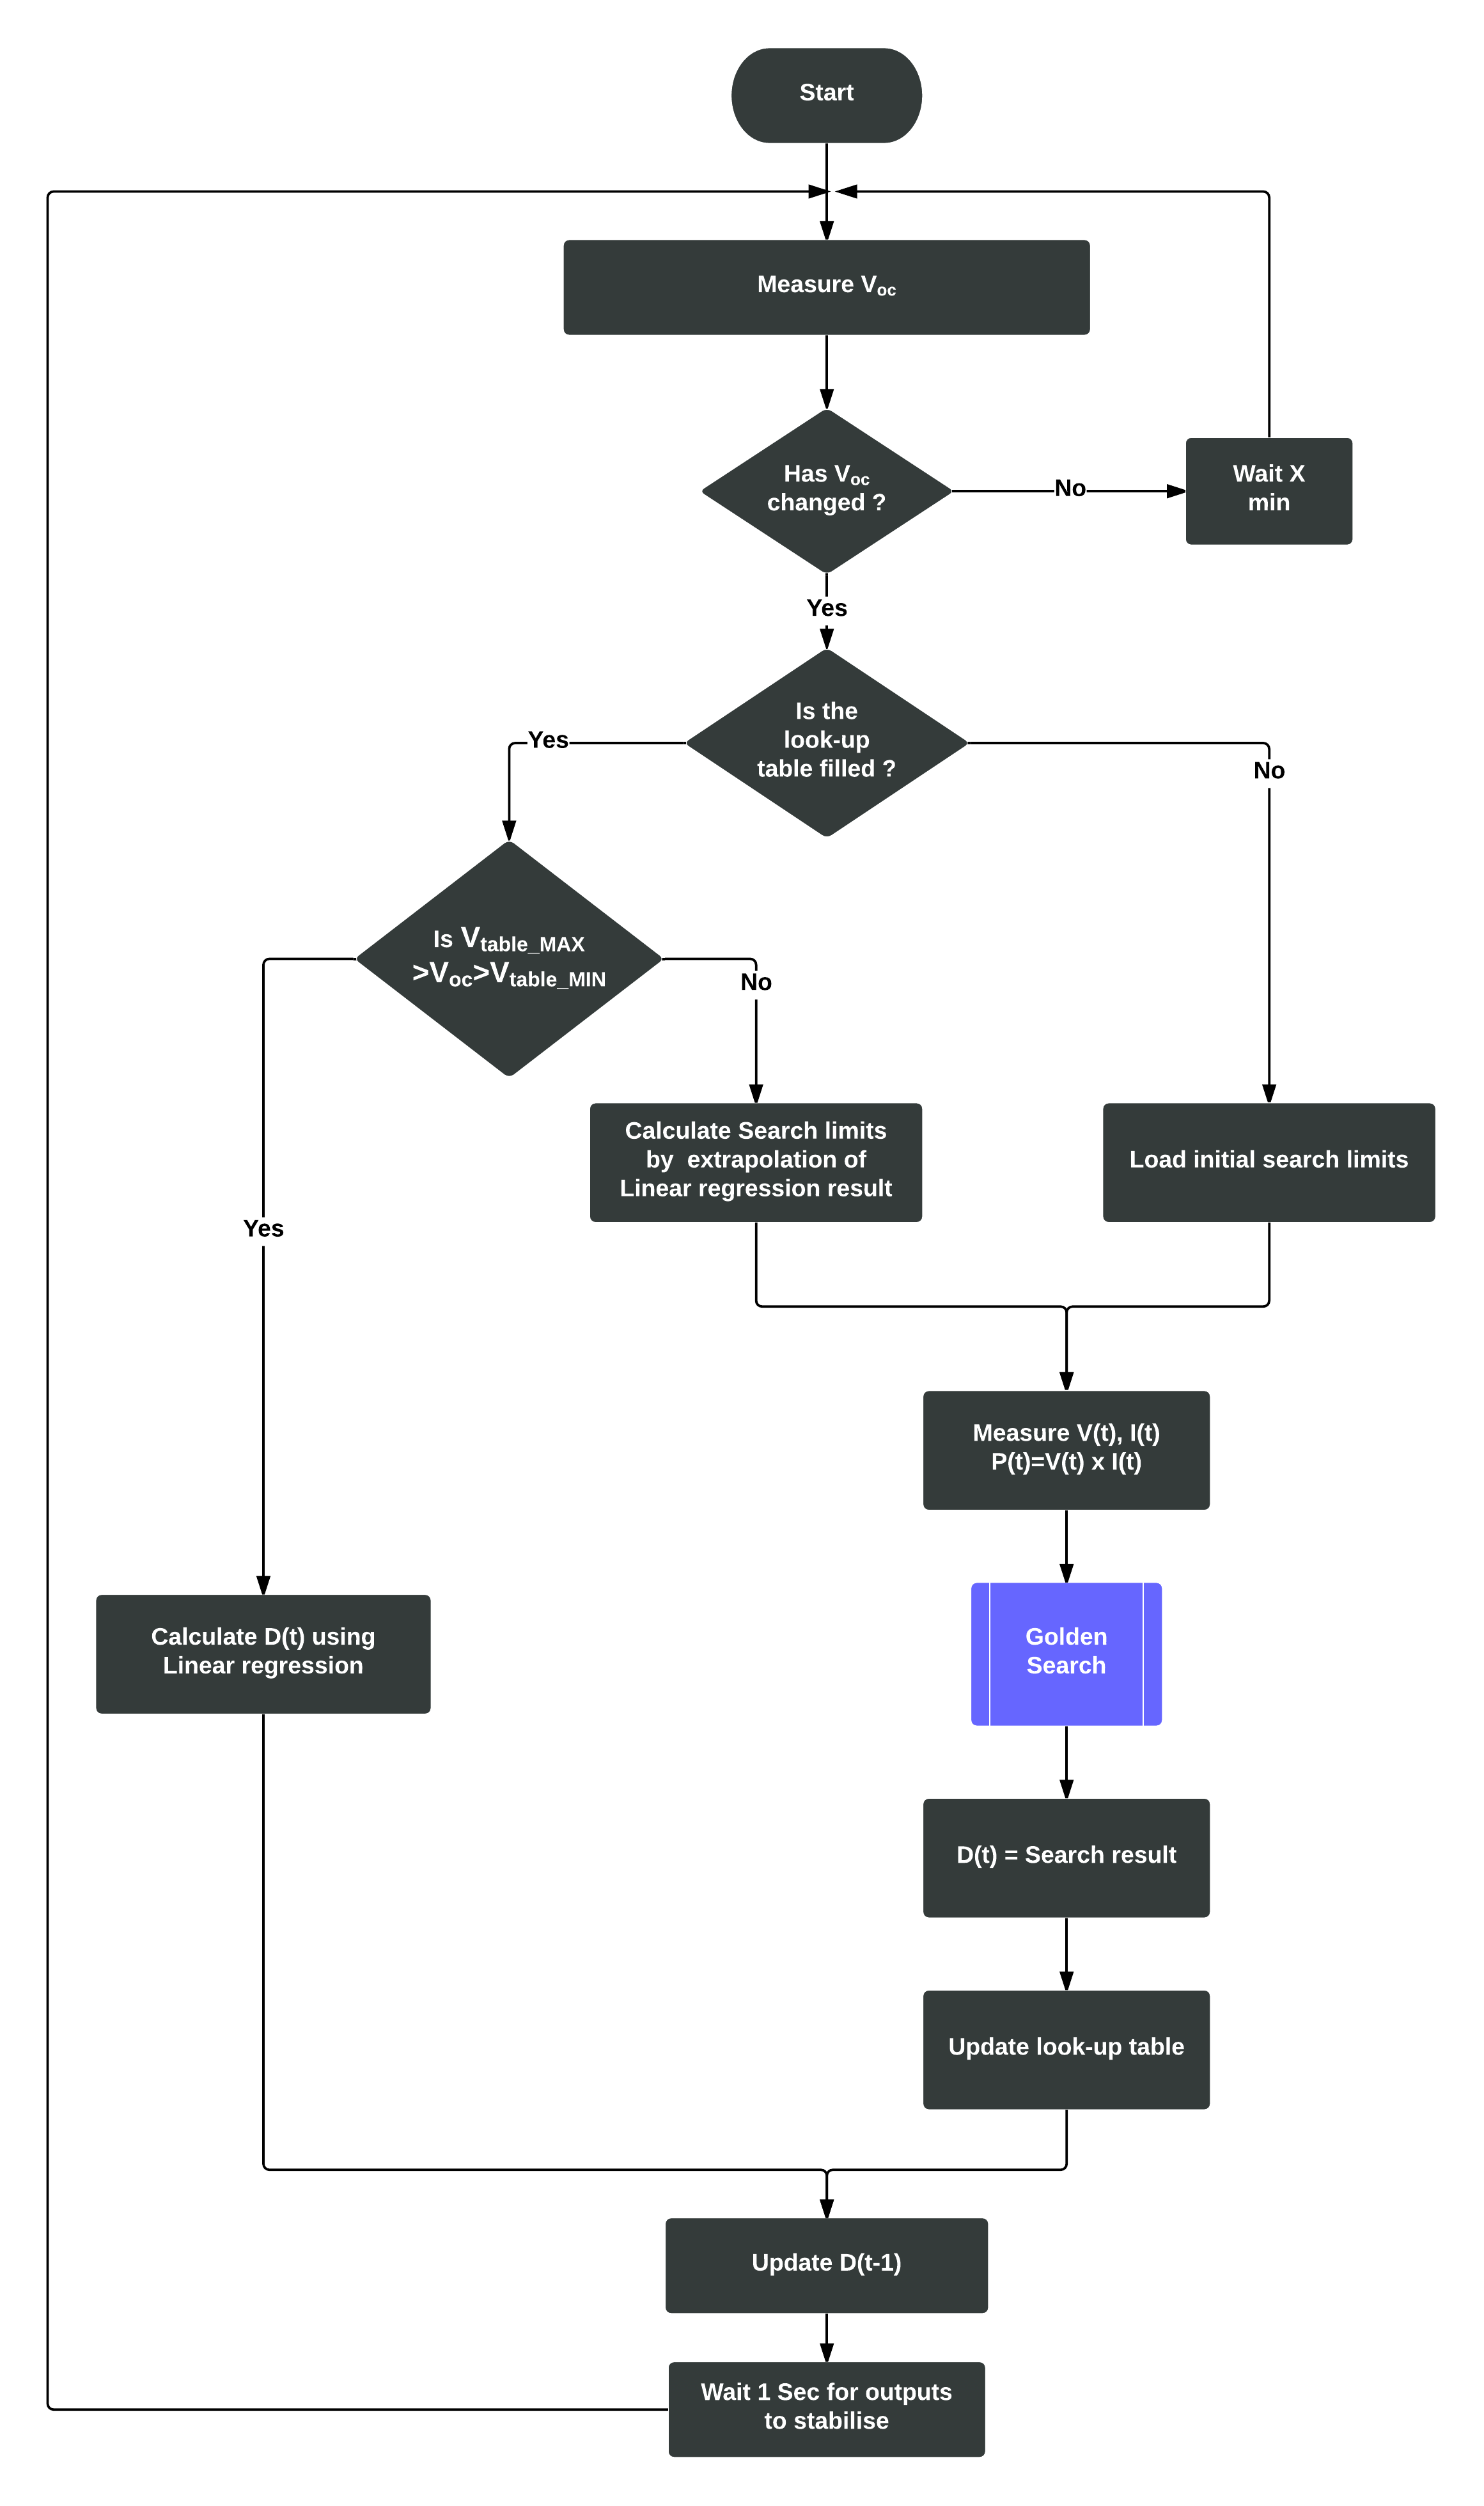
\includegraphics[width=0.9\textwidth]{images/Proposed_Flow}
	   \caption{ Flow chart for Proposed MPPT Algorithm }
	   \label{fig:cyflow}
    \end{center}
  \end{figure}





